\subsection{Statistical analysis methods}
This section shows the methods to obtain a model trained on HHG images, diagnoses and clinical context.
The final model can explain itself via attention maps, which are compared with pathologist annotations.
The pipeline is summarized in

\begin{figure*}
    \centering
    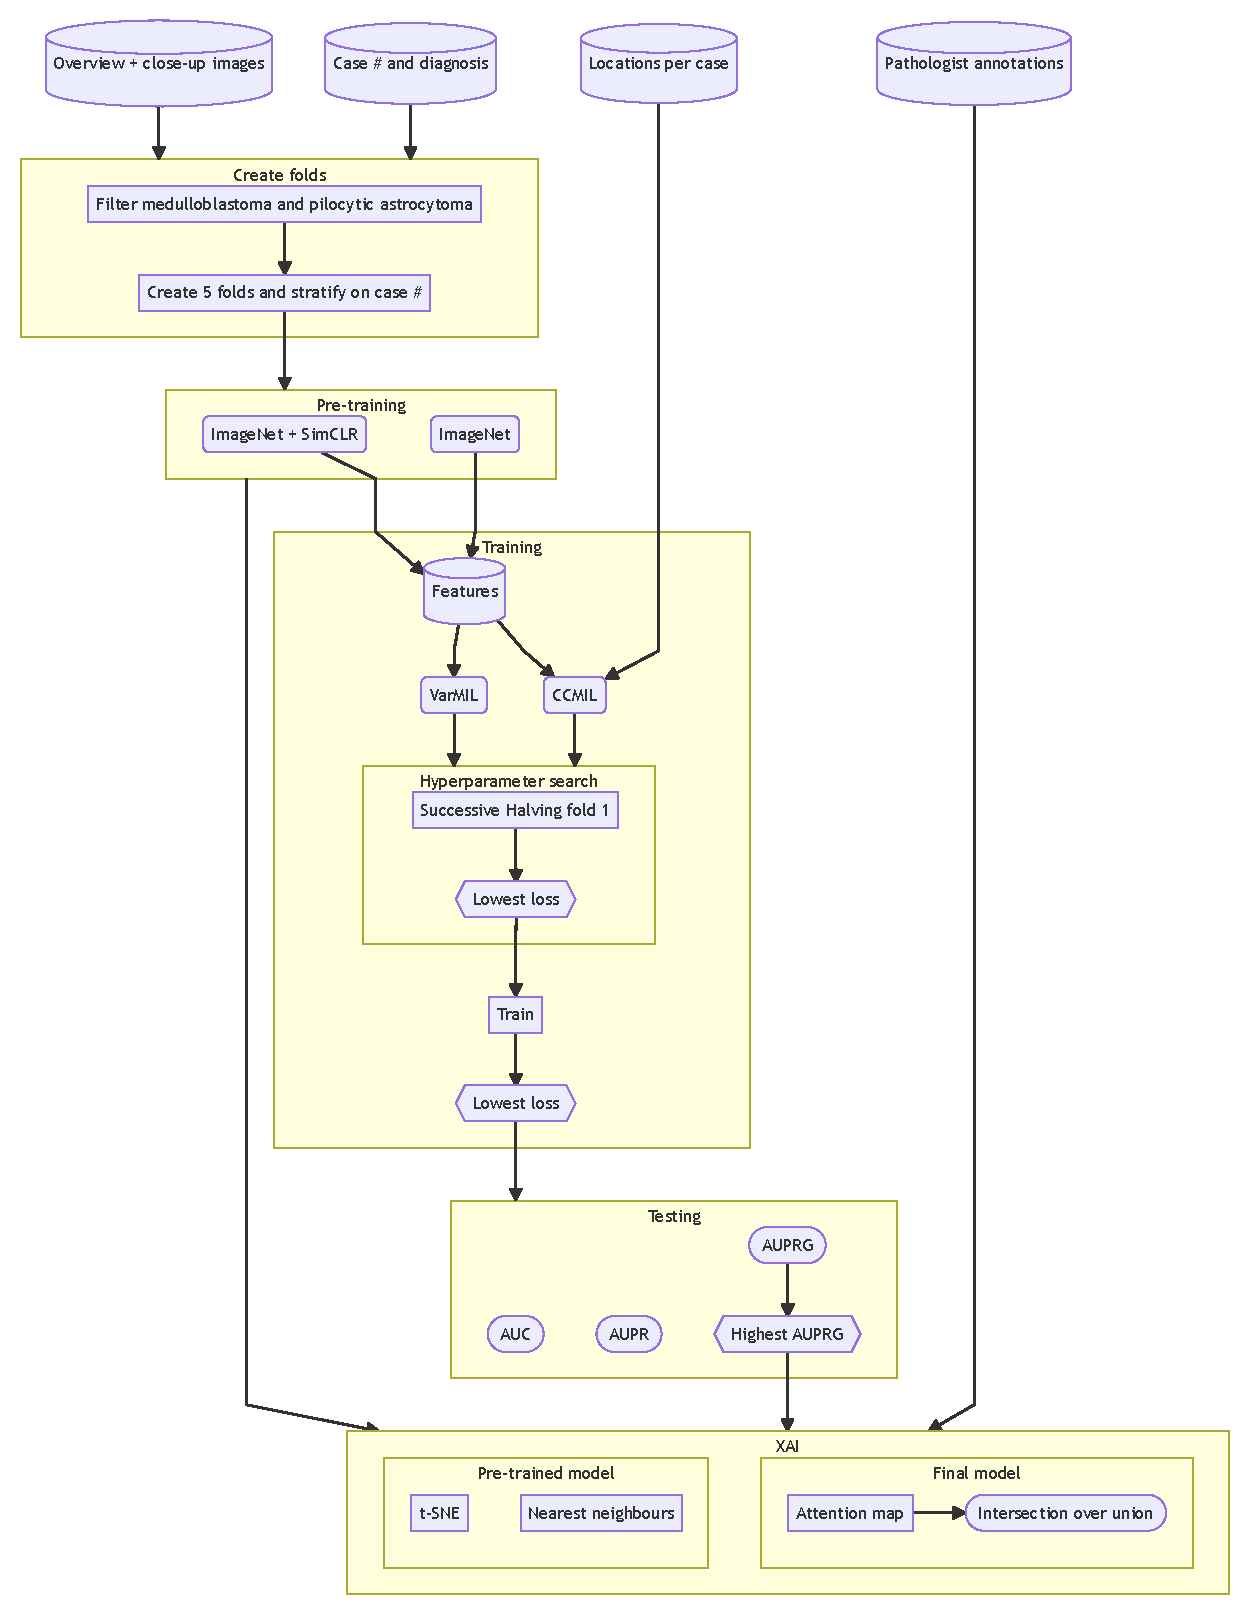
\includegraphics[width=\linewidth]{mermaid/brain/analytical-methods.pdf}
    \caption[Flowchart of training SCLICOM.]{
        Flowchart for training of Self-supervised pre-training and CLInical COntext-aware Multi-instance learning (SCLICOM).
        The images are filtered by diagnosis and divided in splits.
        An ImageNet initialized SimCLR model is trained.
        Features are extracted from this model and an ImageNet initialized model.
        The features are used to train VarMIL and CCMIL models.
        One split for every model is used to search for hyperparameters with which the models are further trained.
        The models are tested on the test set and average precision and $F_1$-score based on thresholds acquired from highest informedness are reported.
        Attention maps are made from the best performing model and compared with pathologist annotations.
    }
\end{figure*}

\subsubsection{Pretraining}
To extract features from the PMC-HHG input tiles, a ImageNet pretrained feature extractor is initialized.
Another feature extractor has an ImageNet pretrained backbone, but is further trained using SimCLR.
Both models are trained for [x] epochs with a batch size of [x].

The pretrained models are internally assessed by visualizing the extracted features in two ways.
First, tiles corresponding to ten nearest neighbours in feature space are compared.
Second, the features are projected with two-dimensional t-SNE after extracting the ten principal components with PCA.
The t-SNE projections are colored by image and case identifier, and diagnosis.

Pretraining is performed on [x] NVIDIA A100 GPUs for [x] days.

\subsubsection{Training}
In total, 20 models are trained using Pytorch Lightning~\cite{Falcon2019}: 4 model definitions and 5 splits.
Using split 1, for every model definition a Successive Halving hyperparameter search is performed on 1 NVIDIA A100 GPU for [x] hours with resources managed by Ray Tune~\cite{Liaw2018} and trials suggested by the grouped multivariate TPE sampler of Optuna~\cite{Akiba2019}.
See [TABLE] for the hyperparameter search settings.
Using the configuration that lead to the model with the lowest validation loss is used for training on all splits for [x] epochs.
The models were trained on [x] NVIDIA A100 GPUs for [x] hours with a bag size of 1, \ie all tiles from one image at a time.

\subsubsection{Testing}
All models from the same initialization are evaluated against a test set.
Average precision and $F_1$-score based on thresholds acquired from highest informedness are reported with a \qty{95}{\percent} CI.
The model with the highest $F_1$-score is selected as the best performing model.
Metrics are calculated by Torchmetrics~\cite{Detlefsen2022}.

\subsubsection{Attention maps}
To verify and to gain knowledge of the inner workings of the model, attention maps are created.
The attention maps are acquired by multiplying the min-max-normalized attention weights with their corresponding tiles.
The maps are compared with tumour annotations from a pathologist.
The IoU of the tumour is reported.
